\chapter{Results and discussion}
\label{chap:results}

Our approach to integrating Embree into ART, as outlined in the previous chapter, was tested on a variety of scene files. This chapter provides an overview and analysis of the performance of our implementation. It is divided into three subsections. Subsection \ref{sec:results_csg} discusses the execution time of ART when rendering scenes CSG. A comparison is drawn between our two approaches for realizing CSG operations with Embree, the initialization of an entire CSG as a user-defined geometry and the traversal through the original scene graph or a dedicated KD tree. We will exclude the provision of results concerning the rendering of CSG through the collection of intersection points and their subsequent evaluation, outlined in Subsection \ref{subsec:apprach1}. This exclusion is due to the immense rendering time resulting from this approach, making it impractical.

Furthermore, we decided to test our implementation on virtual scenes, not necessarily containing CSG, to analyze the overall performance of rendering non-user-defined and user-defined geometries. Section \ref{sec:result_normal} provides the results on various scenes rendered by an hybrid implementation combining the approaches outlined in Subsections \ref{subsec:apprach2} and \ref{subsec:apprach3}. 

Finally, our implementation was tested on scenes, each containing triangle meshes of increasing triangle sizes. The outcome of these experiments is provided and evaluated in Section \ref{sec:result_meshes}.

The following experiments were conducted on an Asus N551JX laptop, which exhibits a quad-core Intel Core i7–4720HQ processor with a frequency of 2.6 GHz and 8 GB of RAM. The images shown in this chapter were rendered in ART with Embree support at a resolution of 700x700, a path length of 20, and a sample size of 128. The image synthesis of these scenes was performed by using the eight available cores of the machine.

\section{Evaluation of our integration for scenes containing CSG}
\label{sec:results_csg}

We tested the functionality of our implementation concerning CSG rendering with Embree on six scenes, which were made publicly available by the developers of ART \footnote{Most of the scenes shown in this chapter can be found in the \texttt{Gallery} folder of the ART repository, which is submitted together with this thesis as an electronic attachment. Scenes or 3D models that are not taken from this folder will be cited.}. All the scenes mentioned in this section contain an infinite sphere, serving as a skydome for illuminating the other scene geometry. 
\\

\noindent For this evaluation, our implementation was tested on the following scenes:
\begin{itemize}
	\setlength\itemsep{0.05em}
	
	\item The scene shown in Figure \ref{fig:csg_shell} consists of a single CSG, a procedurally modeled shell, and multiple cubes aligned to form a checkerboard pattern. The CSG, namely the shell, is composed of a total amount of 2,144 sphere primitives. The shell is modeled by arranging the spheres in spiral form and decreasing order according to their sizes. The largest sphere at the beginning of this sequence of spheres is "subtracted" by the \texttt{SUB} operator from the rest of the spheres. Then, the next largest sphere is "unified" by the \texttt{OR} operator with its preceding sphere in the sequence. This procedure is repeated for the remaining spheres in the sequence.
	
	\item  Figure \ref{fig:csg_orennayar} shows the rendered image of a scene composed of a cylinder serving as the ground on which three so-called \emph{grooved spheres} are placed. The grooves on the sphere result from applying a \texttt{SUB} operator to a group of six tori and the sphere in question.
	The purpose of this scene is to showcase ART's implementation of the Oren–Nayar reflectance model \cite{oren1994generalization} with different roughness grades.
	
	\item We have already encountered the \textbf{Villa Rotonda} scene in Subsection \ref{subsec:apprach1}. As mentioned there, the model of the Villa Rotonda is composed of two CSG with a total number of 1,255 primitives.
		
	\item The scene displayed in Figure \ref{fig:csg_torrancesparrow} is composed of twelve grooved spheres that are placed on three deformed cubes with different heights that together form a staircase. Furthermore, a cylinder serves as the ground. The initial purpose of this particular scene was the demonstration of the implementation of the Torrance–Sparrow reflectance model \cite{torrance1967theory} with varying roughness grades.
	
	\item Figure \ref{fig:csg_plane} shows a rendered image of a scene composed of a cylinder acting as the ground, and a biplane, composed of multiple CSG. The total number of topmost CSG nodes in the scene graph assembled by ART for this particular scene amounts to 28. The total number of geometric primitives of the 28 CSG is 336.
	
	\item Lastly, the rendered scene shown in Figure \ref{fig:csg_locomotive} shows a model of an Austrian steam locomotive. The single model is composed of multiple CSG, a total amount of 354 topmost CSG nodes are present in the scene graph associated with this scene The amount of geometric primitives present in the scene is 3,594.
	
	
\end{itemize}

\begin{figure}
	\centering
	\subfloat[Shell]{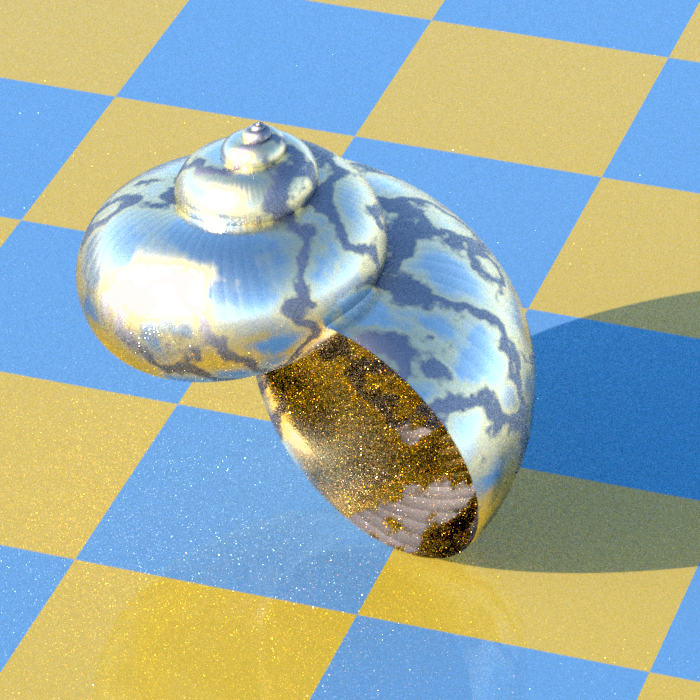
\includegraphics[width=.3\textwidth]{img/4 results/csg/snailEmbree.png}\label{fig:csg_shell}}
	\hfill
	\subfloat[Oren-Nayar Sphreres]{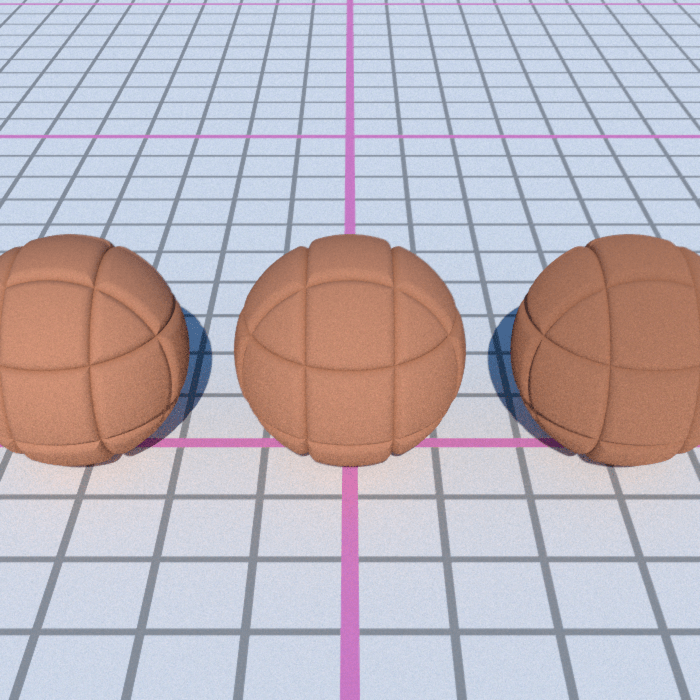
\includegraphics[width=.3\textwidth]{img/4 results/csg/orennayarEmbree.png}\label{fig:csg_orennayar}}
	\hfill
	\subfloat[Villa Rotonda]{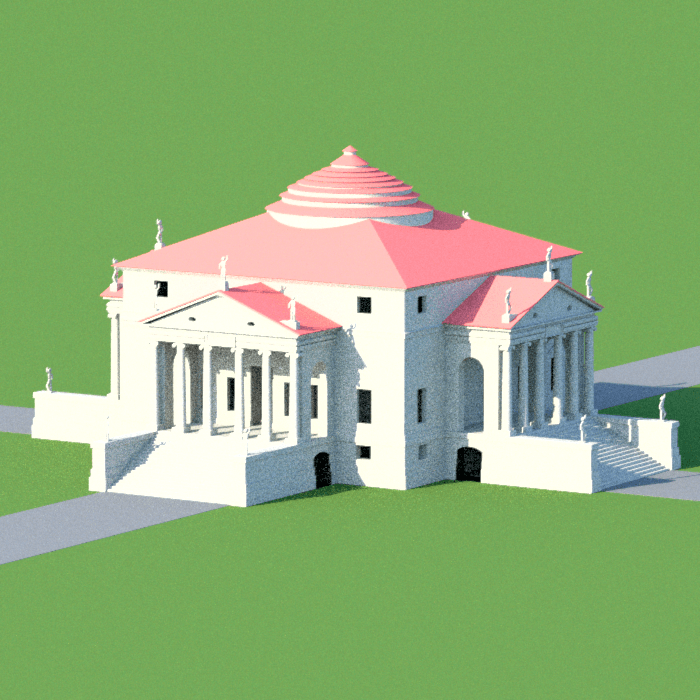
\includegraphics[width=.3\textwidth]{img/4 results/csg/rotondaEmbree.png}\label{fig:csg_rotonda}}
	\\
	\subfloat[Torrance-Sparrow Spheres]{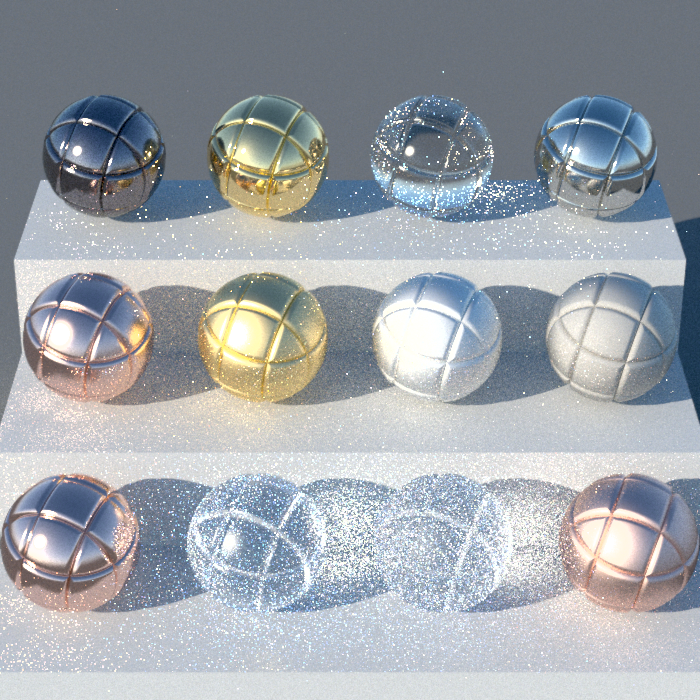
\includegraphics[width=.3\textwidth]{img/4 results/csg/torrancesparrowEmbree.png}\label{fig:csg_torrancesparrow}}
	\hfill
	\subfloat[Parked Biplane]{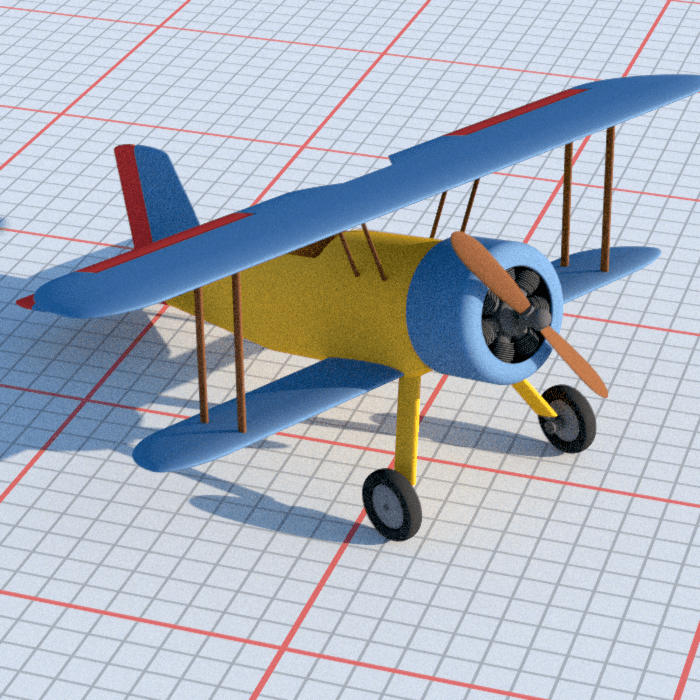
\includegraphics[width=.3\textwidth]{img/4 results/csg/planeEmbree.png}\label{fig:csg_plane}}
	\hfill
	\subfloat[Locomotive]{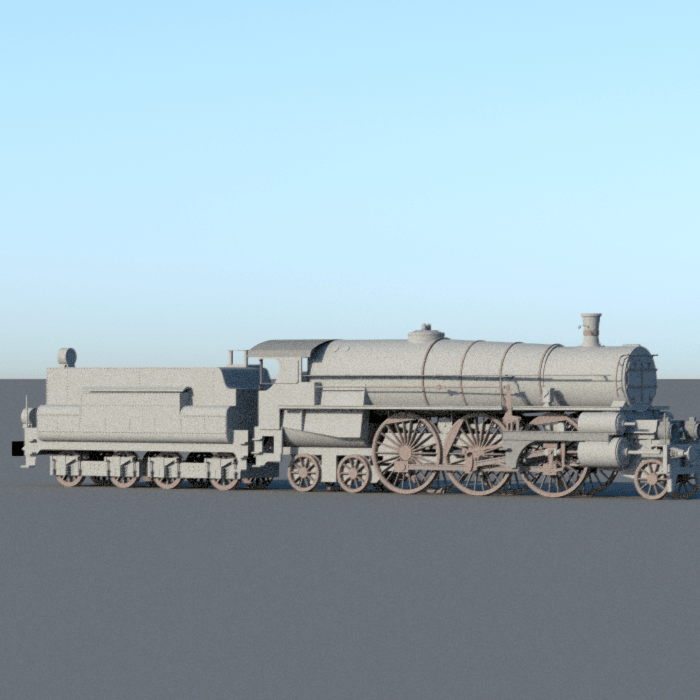
\includegraphics[width=.3\textwidth]{img/4 results/csg/locomotiveEmbree.png}\label{fig:csg_locomotive}}
	
	\caption{Scenes containing CSG, rendered with our implementation. The image of the Villa Rotonda shown in Figure \ref{fig:csg_rotonda} was rendered by traversing KD trees associated with the CSG in this scene. Unfortunately, the issue described in Subsection \ref{subsec:apprach2} remains when rendering the scene by traversing the original scene graph.}
	\label{fig:csg_figures}
\end{figure}

\begin{table}[h]
	\centering
	{\footnotesize\sf
		\begin{tabular}{lrrrrrr}
			\toprule
			Scene & \thead{\texttt{\#}Topmost \\ CSG \\ nodes} & Native ART & \thead{Org scene \\ graph} &  KD tree & \thead{Org scene \\ graph \\ speedup} & \thead{KD tree \\ speedup} \\ 
			\midrule
			Figure \ref{fig:csg_shell} & 1 & 2,611.75 sec & 2,437.81 sec & 4,151.01 sec & 6.66 \% & \textcolor{red}{-58.94 \%}  \\
			Figure \ref{fig:csg_orennayar} & 3 & 791.71 sec & 522.97 sec & 528.77 sec & 33.94 \% & 33.21 \% \\
			Figure \ref{fig:csg_rotonda} & 2 & 738.25 sec & 629.03 sec &  765.44 sec & 14.79 \%  & \textcolor{red}{-3.68 \%}  \\
			\addlinespace % a nice non-intrusive separator of data groups (or final table sums)
			Figure \ref{fig:csg_torrancesparrow} & 12 & 910.56 sec & 896.97 sec & 902.61 sec & 1.49 \%  & 0.87 \% \\
			Figure \ref{fig:csg_plane} & 28 & 522.58 sec & 498.25 sec & 546.79 sec & 4.66 \% & \textcolor{red}{-4.63} \% \\
			Figure \ref{fig:csg_locomotive} & 354 & 312.94 sec & 272.08 sec & 280.83 sec & 13.06 \%  & 10.26 \% \\
			\bottomrule
	\end{tabular}}
	\caption{Comparison between the performances of Native ART and ART with Embree support. The performance of both methods of traversing the original scene graph and traversing the dedicated KD tree is compared to the performance of Native ART.}
	\label{tab:csg}
\end{table}

As can be seen in Table \ref{tab:csg}, the \todo{do}

\subsubsection{Special case: Rendering CSG composed of triangle meshes}

\begin{figure}[h]
	\centering
	\subfloat[Scene rendered with native ART by traversing the internal KD tree.]{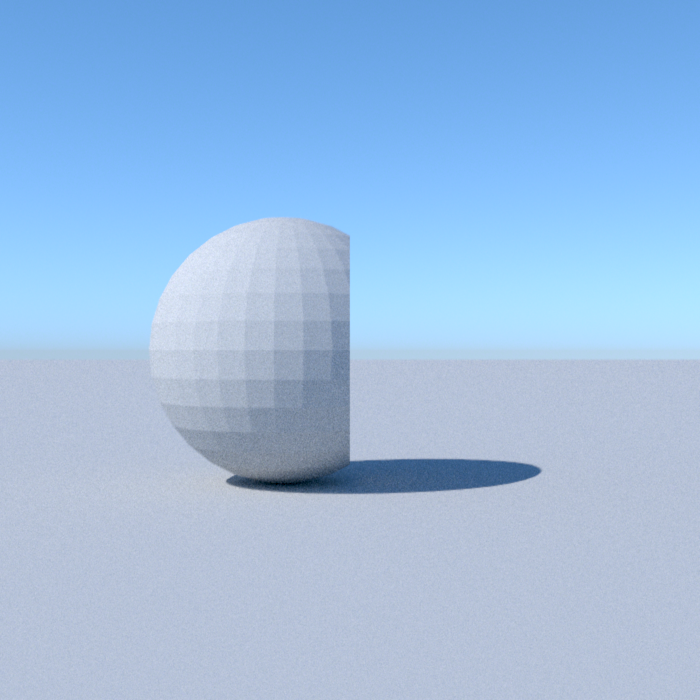
\includegraphics[width=.4\textwidth]{img/3 approach/spheresEmbree.png}\label{fig:csg_mesh_spheres}}
	\hfil
	\subfloat[Artifact in the scene rendered with the approach outlined in this section.]{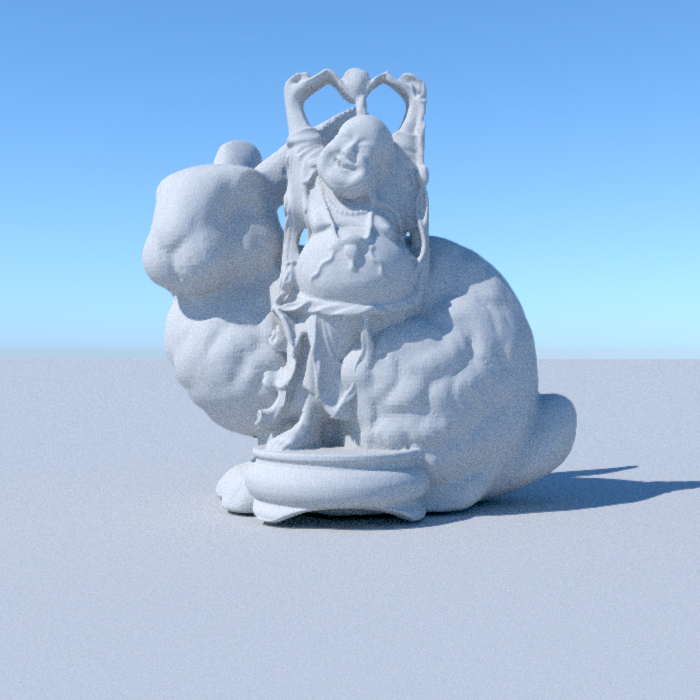
\includegraphics[width=.4\textwidth]{img/4 results/csg/meshCSGEmbree.png}\label{fig:csg_mesh_bunny_buddha}}
	\caption{CSG composed of triangle meshes. The figures show a scene with two spheres described as triangle meshes. The right sphere is "subtracted" from the left sphere via the Boolean set operation \texttt{OR}. The scene can be regarded as the counterpart of the scene shown in Figure \ref{fig:csg_sub} for triangle mesh primitives.}
	\label{fig:csg_mesh_results}
\end{figure}

\begin{table}[h]
	\centering
	{\footnotesize\sf
		\begin{tabular}{lrrrrr}
			\toprule
			Scene  & \thead{Native ART \\ Preparation} & \thead{Native ART \\ Ray \\ Tracing} & \thead{Embree \\ Preparation} & \thead{Embree \\ Ray Tracing} & \thead{Ray Tracing \\ Speedup} \\ 
			\midrule
			Figure \ref{fig:csg_mesh_spheres} & 0.09 sec & 237.25 sec & 0.09 sec & 284.86 sec & \textcolor{red}{-20.07 \%} \\
			Figure \ref{fig:csg_mesh_bunny_buddha} & 4.58 sec & 376.20 sec & 61.82 sec & 709.77 sec  & \textcolor{red}{-88.67 \%} \\
			\bottomrule
	\end{tabular}}
	\caption{Comparison between the performances of Native ART and ART with Embree support. The time needed for preparing the ray tracing process by constructing the internal acceleration data structures and the time needed for the ray tracing process itself.}
	\label{tab:csg_mesh}
\end{table}

For testing our implementation on scenes that contain CSG, which are composed of triangle meshes, we modeled two scenes. Figure \ref{fig:csg_mesh_spheres} shows the rendered image of a scene, composed of a quadrangle and two spheres that are described by triangle meshes. The right sphere is "subtracted" from the left sphere by applying the difference set operation. Figure \ref{fig:csg_mesh_bunny_buddha} shows the rendered image of a scene that contains again of a quadrangle, and two triangle meshes provided by the Stanford 3D Scanning Repository \cite{plyRepo}, namely the Stanford Bunny, composed of 69,451 triangles and the Happy Buddha, composed of 1,087,716 triangles. The results are shown in Table \ref{tab:csg_mesh}.
As described in Subsection \ref{subsec:apprach2}, ray tracing these types of CSG is not possible with our approach of traversing the original scene graph. Therefore, the results shown refer to the approach of traversing individual KD trees associated with the CSG.

The results in the table indicate a significant decrease in ray tracing performance when rendering CSG composed from triangle meshes. This drop-off can be explained the following way: Embree was originally developed for rendering scenes containing complex geometry, being described by a high number of primitives. Therefore, it does not perform well with scenes containing a small number of geometries. In our scenes, only two geometries are present, a plane and the entire CSG. Furthermore, the combining of Embree's BVHs and ART's internal KD trees for such simple scenes does not accelerate the intersection calculation process. It, in fact, complicates it.

We do not recommend using our approach to render CSG composed of triangle meshes at the current stage. 


\section{Hybrid implementation and evaluation}
\label{sec:result_normal}

After examining the results of our tests concerning the rendering of CSG described in the previous section, we decided to abandon our approach of calculating the intersection points by traversing a KD tree associated with the CSG in question. This is because the traversal of the original scene subgraph rooted at the topmost CSG node is faster. For now, we accept the drawback concerning the Villa Rotonda scene missing its roof as a known issue (as outlined in Subsection \ref{subsec:apprach2}), since we strongly believe that this issue is rather connected to the scene graph traversal than to the functionality concerning Embree. Finding an adequate solution to resolve this issue will be a part of our future work.

However, we cannot completely abandon the approach of building and traversing individual KD trees for CSG since scenes with CSG that are composed of at least one triangle mesh strictly depend on the KD trees.

Therefore, our final implementation of the facilitation of CSG rendering with Embree consists of a hybrid combination between Approach 2 and Approach 3: Before the actual image synthesis procedure in ART, the scene graph is assembled. When, during this step, a topmost CSG node corresponding to a CSG that is constructed by at least one triangle mesh, a flag associated with the CSG is activated. Whenever such a flag is activated for a CSG in question, the internal KD tree for the triangle mesh primitive is built and the KD tree for the CSG according to Approach 3. If such a CSG, being constructed of at least one triangle mesh, is intersected by a ray during the ray tracing procedure, the intersections between ray and CSG are calculated by the traversal of the associated KD tree.

The intersection calculations between rays and CSG that are not constructed of at least one triangle mesh, are calculated by traversal of the scene subgraph rooted at the topmost CSG node corresponding to the particular CSG, according to Approach 2.

This section provides results of tests conducted with this final implementation.
\\

\noindent In the following, we provide an overview of the scenes used for testing the overall performance of ART with Embree support:
\begin{itemize}
	\setlength\itemsep{0.05em}
	
	\item MacBeth ColorChecker - 26 geom
	
	\item Cornell Box with image - 20 geom
	
	\item glowing spheres - 13 geom
	
	\item Figure \ref{fig:skydome} shows an image that was originally published in the research article \citetitle{wilkie2013predicting} \cite{wilkie2013predicting}.
	
	- 10 x 13 for grooved spheres, 1 mirror sphere, colorchecker, traingle mesh, cylinder
	
	
\end{itemize}


\begin{figure}
	\centering
	\subfloat[Macbeth ColorChecker]{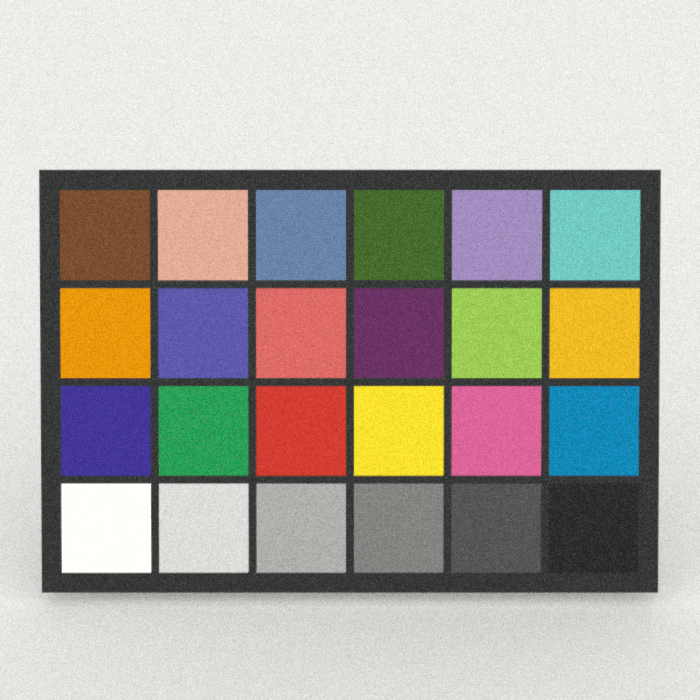
\includegraphics[width=.3\textwidth]{img/4 results/normal/chartEmbree.png}\label{fig:chart}}
	\hfill
	\subfloat[Cornell box with texture mapping]{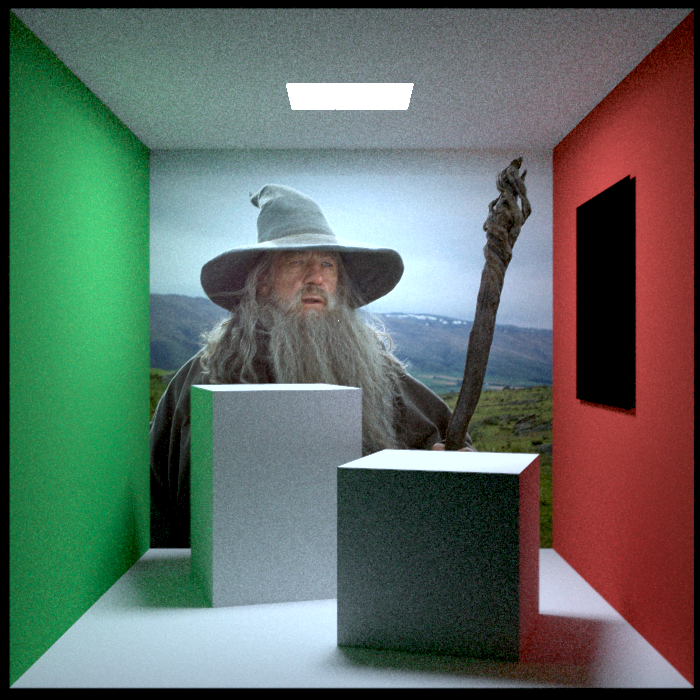
\includegraphics[width=.3\textwidth]{img/4 results/normal/imagemapEmbree.png}\label{fig:gandalf}}
	\hfill
	\subfloat[Glowing spheres]{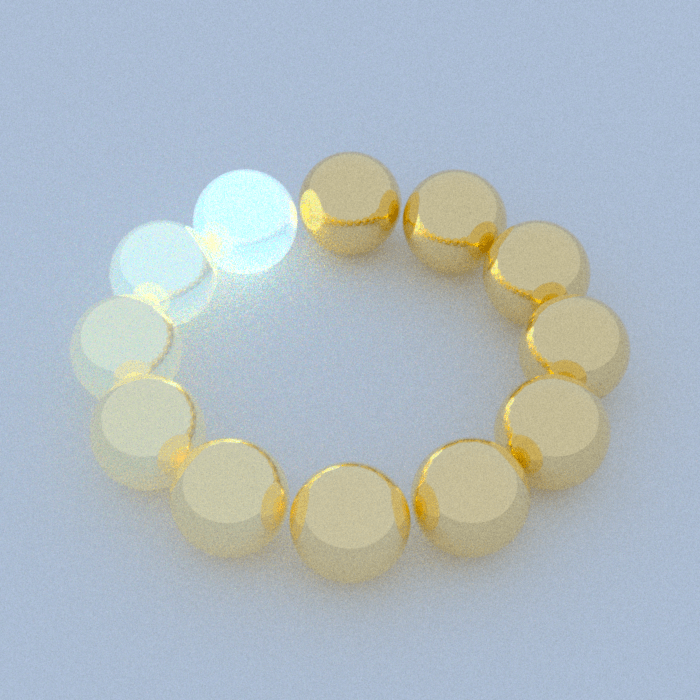
\includegraphics[width=.3\textwidth]{img/4 results/normal/glowEmbree.png}\label{fig:glow}}
	\\
	\subfloat[Exoplanet scene]{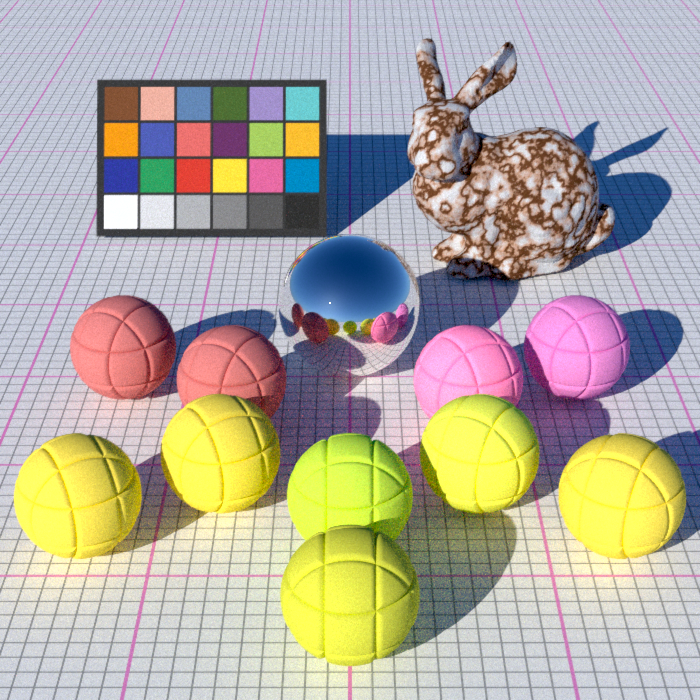
\includegraphics[width=.7\textwidth]{img/4 results/normal/skydomeEmbreeFinal.png}\label{fig:skydome}}

	
	\caption{Scenes from the gallery of the ART repository.}
	\label{fig:scenes}
\end{figure}


\begin{table}
	\centering
	{\footnotesize\sf
		\begin{tabular}{lrrrr}
			\toprule
			Scene & \Verb!#!Geometries & Native ART & Embree & Speedup \\ 
			\midrule
			Figure \ref{fig:chart} & 26 & 196.34 sec & 213.15 sec & \textcolor{red}{-8.56 \%} \\
			Figure \ref{fig:gandalf} & 20 & 454.60 sec & 229.73 sec & 49.47 \% \\
			Figure \ref{fig:glow} & 13 & 401.27 sec & 225.29 sec & 43.86 \%  \\
			Figure \ref{fig:skydome} & 38 & 761.25 sec & 621.96 sec & 18.30 \% \\
			\bottomrule
	\end{tabular}}
	\caption{An example table. Table caption should clearly explain how to interpret the data in the table. Use some visual guide, such as boldface or color coding, to highlight the most important results (e.g., comparison winners).}
	\label{tab:scenes}
\end{table}



\begin{figure}
	\centering
	\subfloat[Macbeth ColorChecker]{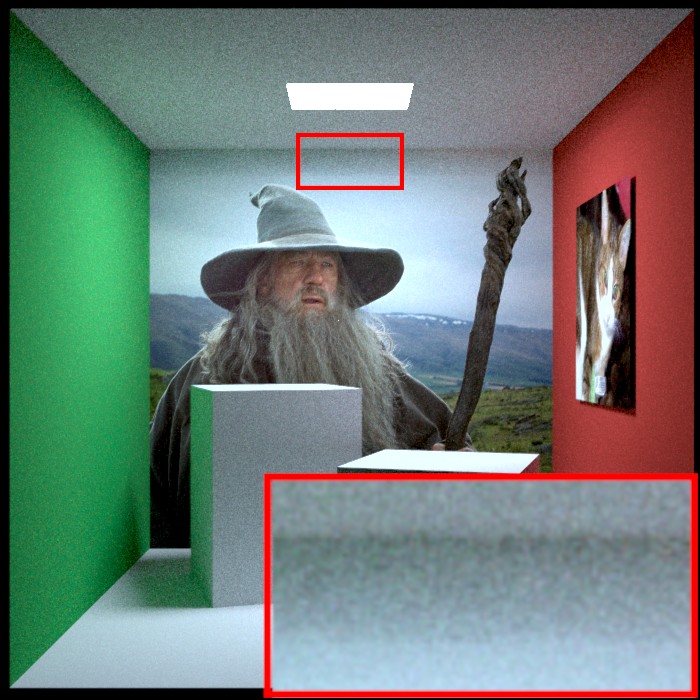
\includegraphics[width=.45\textwidth]{img/4 results/normal/imagemapEmbreeDetail.png}\label{fig:gandalf_embree}}
	\hfill
	\subfloat[Cornell box with texture mapping]{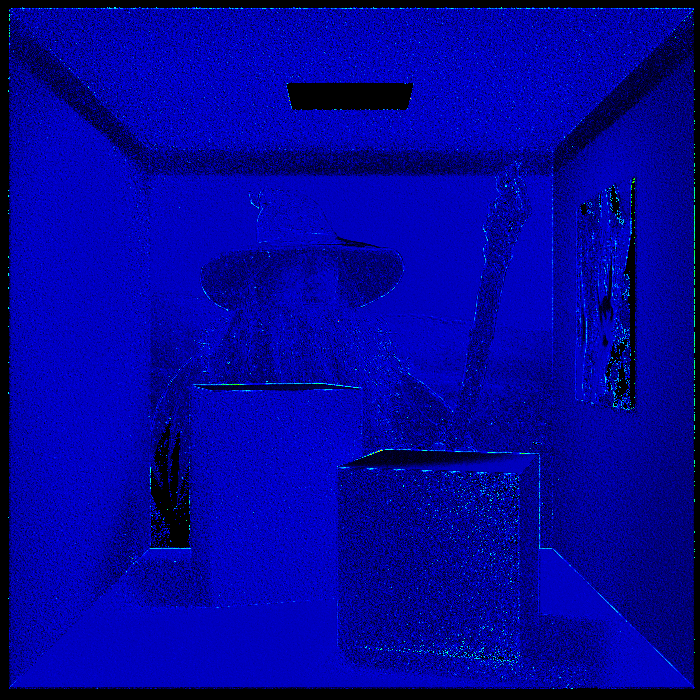
\includegraphics[width=.45\textwidth]{img/4 results/normal/differenceEmbreeNormal.png}\label{fig:difference_embree}}
	\\
	\subfloat[Glowing spheres]{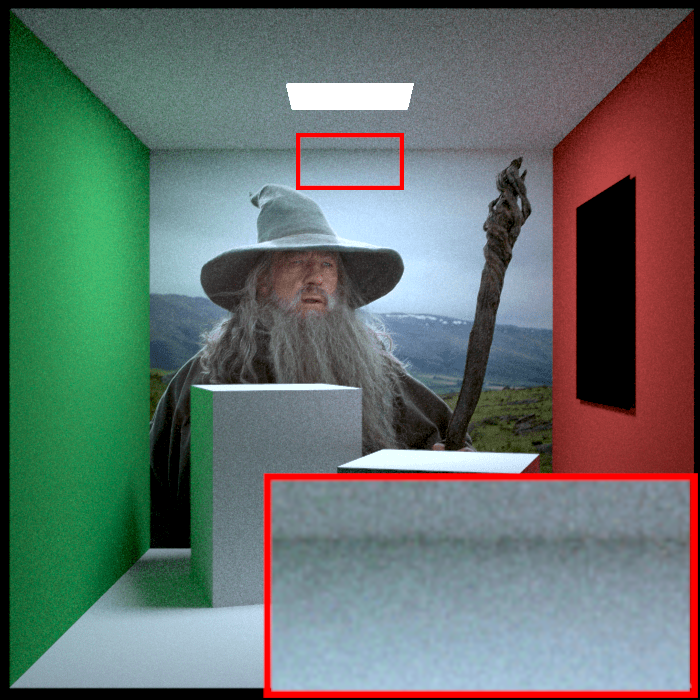
\includegraphics[width=.45\textwidth]{img/4 results/normal/imagemapEmbreeUserDetail.png}\label{fig:gandalf_embree_user}}
	\hfill
	\subfloat[Exoplanet scene]{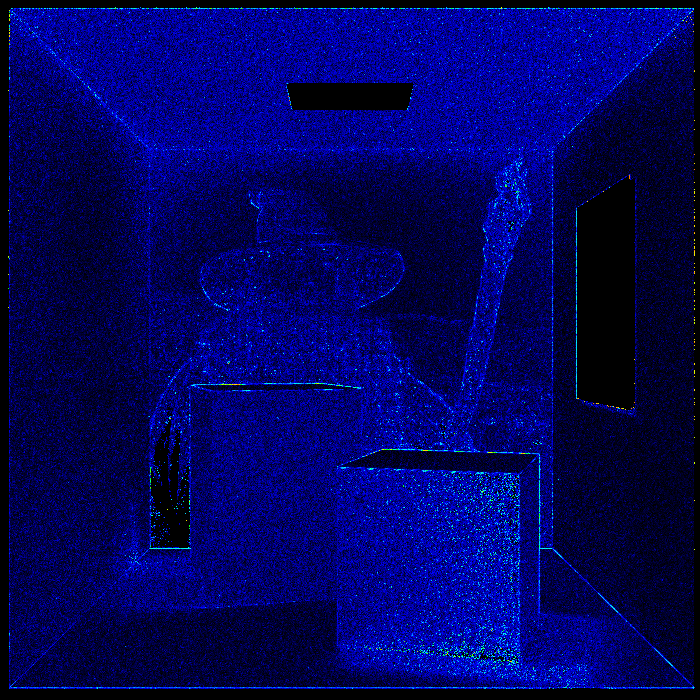
\includegraphics[width=.45\textwidth]{img/4 results/normal/differenceUserNormal.png}\label{fig:difference_embree_user}}
	
	
	\caption{Scenes from the gallery of the ART repository.}
	\label{fig:res_gandalf_issue}
\end{figure}


\section{Evaluation of our implementation for scenes containing triangle meshes}
\label{sec:result_meshes}

Since the rendering of large triangle meshes is the most crucial use case for Embree, we tested our implementation on various triangle meshes.

Each scene shown in Figure \ref{fig:mesh_scenes} is composed of a quadrangle serving as ground, an infinite sphere acting as a sky dome for illumination and a single triangle mesh, that are loaded from a PLY file and assigned with a material associated with the Torrance–Sparrow reflectance model.
\\

\noindent The following models were used for our tests:
\begin{itemize}
	\setlength\itemsep{0.05em}
	
	\item The \textbf{Utah Teapot} (4,032 triangles), provided by Ben Houston \cite{teapot}, shown in Figure \ref{fig:mesh_teapot}
	\item The \textbf{Stanford Bunny} (69,451 triangles), provided by the Stanford PLY repository, shown in Figure \ref{fig:mesh_bunny}
	\item \textbf{Michelangelo's David} (366,011 triangles), provided by Jerry Fisher \cite{david}, shown in Figure \ref{fig:mesh_mike}
	\item The \textbf{Happy Buddha} (1,087,716 triangles), provided by the Stanford PLY repository, shown in Figure \ref{fig:mesh_buddha}
	\item The \textbf{Asian Dragon} (7,219,045 triangles), provided by the Stanford PLY repository, shown in Figure \ref{fig:mesh_dragon}
	\item \textbf{Lucy} (28,055,742 triangles), provided by the Stanford PLY repository, shown in Figure \ref{fig:mesh_lucy}
\end{itemize}


\begin{figure}
	\centering
	\subfloat[Utha Teapot]{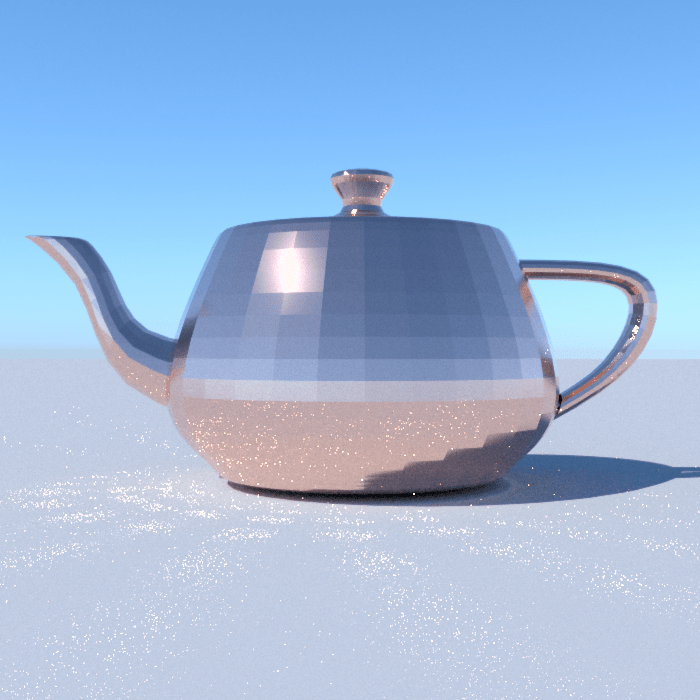
\includegraphics[width=.3\textwidth]{img/4 results/ply/teapotEmbree.png}\label{fig:mesh_teapot}}
	\hfill
	\subfloat[Stanford Bunny]{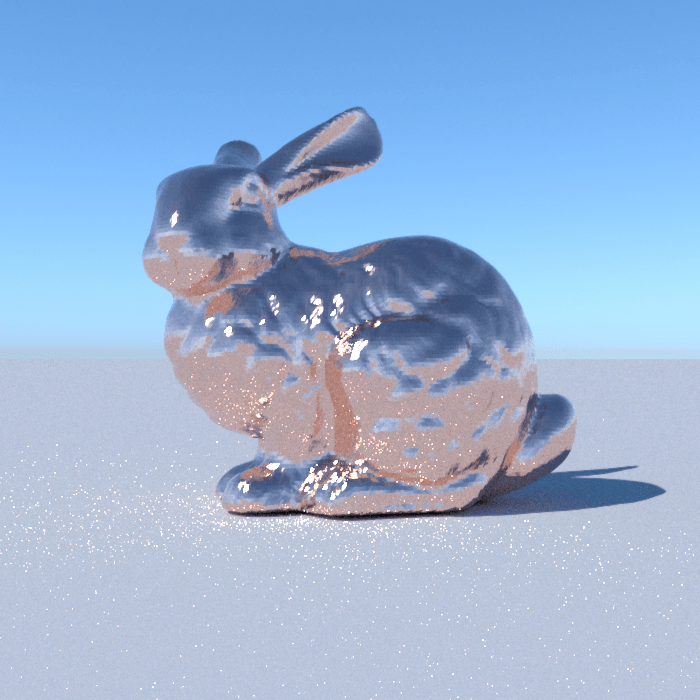
\includegraphics[width=.3\textwidth]{img/4 results/ply/bunnyEmbree.png}\label{fig:mesh_bunny}}
	\hfill
	\subfloat[Michelangel's David]{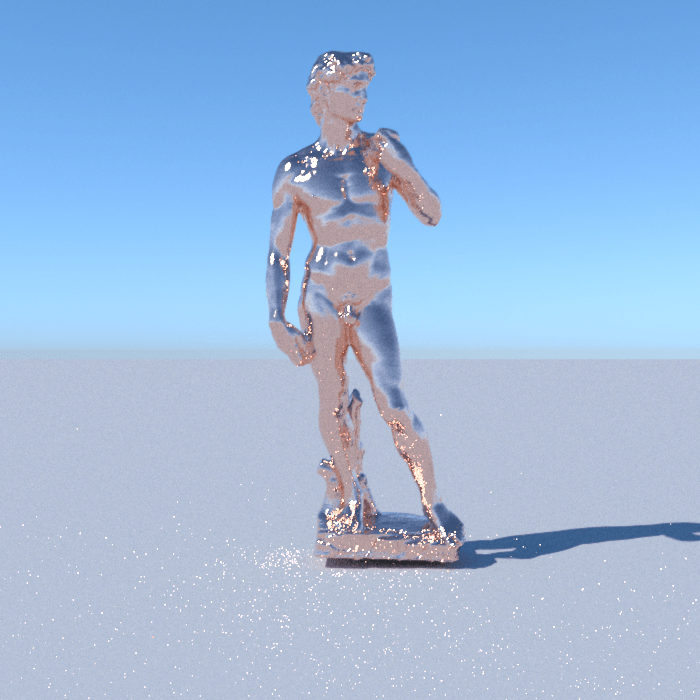
\includegraphics[width=.3\textwidth]{img/4 results/ply/michelangeloEmbree.png}\label{fig:mesh_mike}}
	\\
	\subfloat[Happy Buddha]{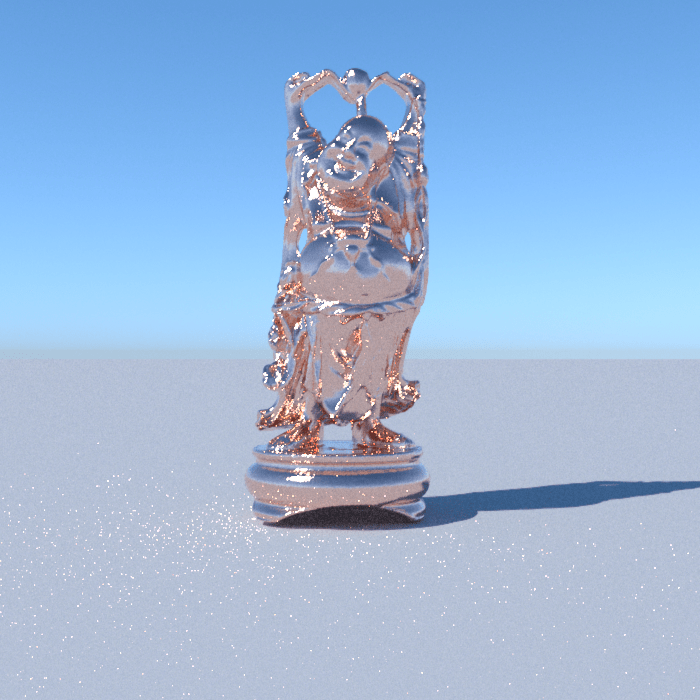
\includegraphics[width=.3\textwidth]{img/4 results/ply/bhuddaEmbree.png}\label{fig:mesh_buddha}}
	\hfill
	\subfloat[Asian Dragon]{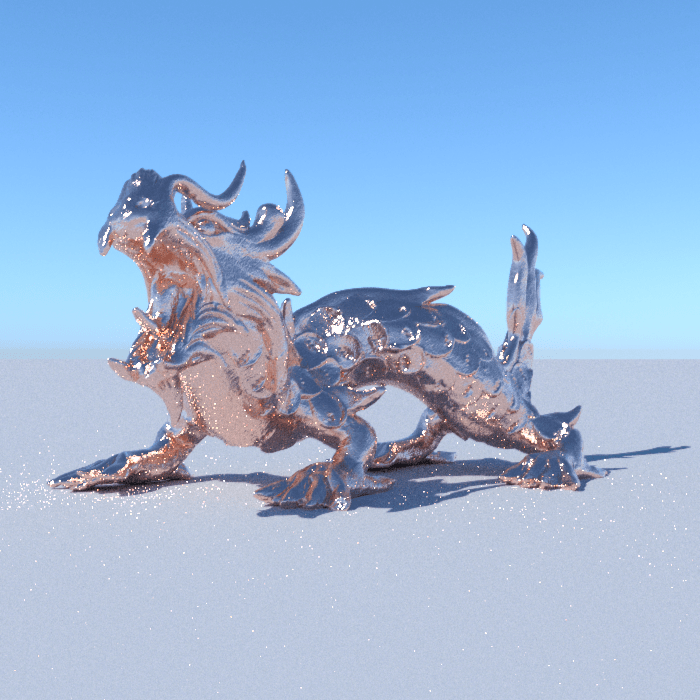
\includegraphics[width=.3\textwidth]{img/4 results/ply/dragonEmbree.png}\label{fig:mesh_dragon}}
	\hfill
	\subfloat[Lucy]{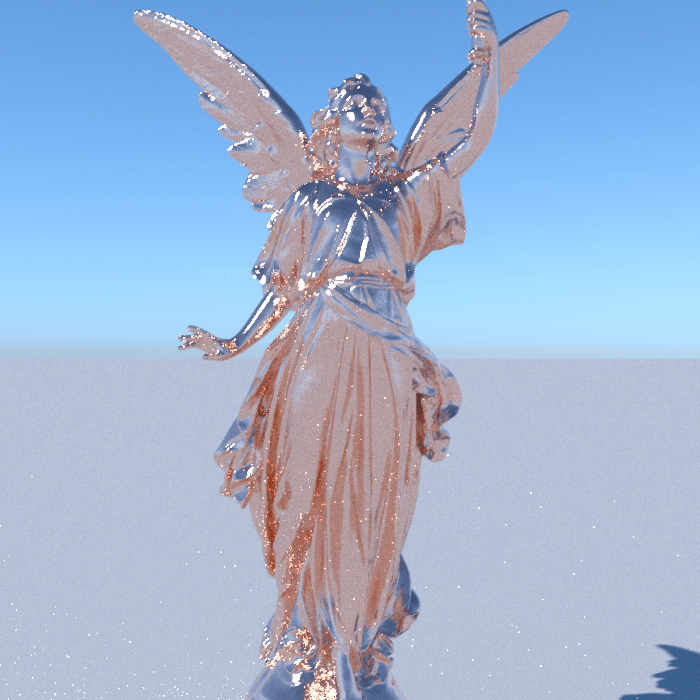
\includegraphics[width=.3\textwidth]{img/4 results/ply/lucyEmbree.png}\label{fig:mesh_lucy}}
	
	\caption{Scenes for triangle meshes}
	\label{fig:mesh_scenes}
\end{figure}


\begin{table}
	\centering
	{\footnotesize\sf
		\begin{tabular}{lrrrrr}
			\toprule
			Scene  & \thead{Native ART \\ Preparation} & \thead{Embree \\ Preparation}  & \thead{Native ART \\ Ray Tracing} & \thead{Embree \\ Ray Tracing} &  \thead{Ray Tracing \\ Speedup}\\ 
			\midrule
			Figure \ref{fig:mesh_teapot} & 0.29 sec & 0.04 sec & 353.83 sec & 304.26 sec &  14.01 \% \\
			Figure \ref{fig:mesh_bunny}  & 4.28 sec & 0.25 sec & 379.02 sec & 305.00 sec &  19.53 \% \\
			Figure \ref{fig:mesh_mike} & 18.40 sec & 1.85 sec &  302.52 sec & 254.03 sec &  16.03 \%  \\
			\addlinespace % a nice non-intrusive separator of data groups (or final table sums)
			Figure \ref{fig:mesh_buddha}  & 57.28 sec & 6.48 sec & 351.92 sec & 276.00 sec &  21.57 \% \\
			Figure \ref{fig:mesh_dragon} & (no data)  & 64.43 sec & (no data) & 304.29 sec & (no data)  \\
			Figure \ref{fig:mesh_lucy}  & (no data) & 302.19 sec & (no data) & 327.59 sec & (no data)  \\
			\bottomrule
	\end{tabular}}
	\caption{An example table. Table caption should clearly explain how to interpret the data in the table. Use some visual guide, such as boldface or color coding, to highlight the most important results (e.g., comparison winners).}
	\label{tab:mesh}
\end{table}

The results in Table \ref{tab:mesh} show a general increase of the performance of ART when supported by Embree. Another advantage of our implementation compared to Native ART is that the time needed to prepare the scene for ray tracing decreased since we omit the construction of KD trees for triangle meshes.

However, we could not render the Asian Dragon and Lucy meshes with Native ART on our local machine. This is because these meshes are large, and so is ART's internal KD tree for grouping the individual triangles into spaces bound by split planes. For triangle meshes composed of a number of triangles higher than a certain threshold, the required memory needed for the construction of the mesh KD tree exceeds the available system memory, which, in our case, results in a termination of the program by the Linux kernel.

At this point, we would like to emphasize that through our implementation, the rendering of such large triangle meshes is possible on machines comparable to the one we used for our tests.
